\documentclass{exam}
\usepackage[utf8]{inputenc}
\usepackage{graphicx}
\usepackage{dblfloatfix}
\usepackage{amsmath}
\makeatletter
\def\@seccntformat#1{%
  \expandafter\ifx\csname c@#1\endcsname\c@section\else
  \csname the#1\endcsname\quad
  \fi}
\makeatother
% naam punten
\extraheadheight[1.5cm]{1cm}
\usepackage[toc,page]{appendix}
%header
\runningheader{}{De verborgen hints }{}
\runningfooter{Hints }{Astrid Quiz 2019 }{}



\begin{document}

\begin{titlepage}
\center

\includegraphics[scale=0.08]{astrid}
\linebreak
\linebreak
\linebreak

\vspace{1em}{\huge \bfseries  CodeBook: De Verbogen Hints }
\linebreak

\vspace{1em}{\LARGE  Door cultuur home Astrid} 
            \linebreak
\vspace{1em}{\large 26 november Astrid}
	\begin{center}
	\fbox{\fbox{\parbox{5.5in}{\centering Door heen de quiz zijn er weer tal van verborgen hints verstopt geweest.\\ Eens benieuwd naar al die gemiste kansen en domme verwijzingen?\\ WAARSCHUWING, sommige van deze hints kunnen vergezocht lijken :)}}}
	\end{center}
\end{titlepage}
\newpage
\section*{Voorwoord}
Namens het volledige Home Astrid presidium danken wij u voor uw deelname!\\ \\
We hopen dat iedereen een aangename avond heeft en wensen iedereen zeer veel succes. De hoofdprijzen zijn paintball en twee wijnproeverijen, maar wees gerust de trootsprijzen zijn even leuk of zelfs leuker! Daarvoor willen we onze sponser de Makro bedanken.\\ \\
Een kladblad wordt bij elke tafel ronde gegeven. Aan de bar is er de mogelijkheid om meer kladbladeren te vragen.\\ \\
P.S.\\ \\
Leuk weetje, ookal vonden sommige de vorige quiz moeilijk, het puntengemiddelde was $64,2\%$ per ronde.\\ \\
Vergeet zeker de regels niet te lezen!\\ \\ \\ \\
Cultuur Lemmy en Tibo
\newpage
\section*{Gotcha already!}
Een aandachtige astrid quizzer zal er opgelet hebben dat de vorige quiz geen voorwoord had, wel dit was natuurlijk niet zonder reden.\\ \\Het is niet enkel een informatieve voorwoord, maar het PS. gedeelte wijst nog eens extra naar vorig jaar, met de bedoeling dat men nog extra ging opletten op de verschillen tussen de twee quiz-edities. En ook, om eerlijk te zijn, voor het gezaagd af te zijn dat onze quiz te moeilijk was.\\ \\
Maar ook voor de mensen die niet konden meedoen met de vorige quiz, (enig echt excuus was doodvallen), hebben een cadeautje gekregen. Als je erop gelet had dat het percentage een extra lang kommagetal heeft. dan wist je dat dit wel een antwoord op één van de vragen kon zijn...
\section*{Great men are not born great, they grow great...}
Ook in de poster zaten er een paar hints verwerkt. Allereerst kon men het lettertype en poster layout linken aan de film-klassieker de godfather. Sinds wij afgebeeld zijn als de "acteurs", kan je de schiftingsvraag al beginnen te raden.\\ \\ Als extraatje zat het woord 3D ook nog eens verwerkt in de kakkerlak. Dit was de hint voor de puzzelronde (oplossing is ook toegevoegd).
\section*{The old one}
Sommmige hadden het vorige quiz door, soms door onhandig te zijn en hun bier te morsen.\\ \\Op elke tafel was er verborgen hint verstopt, namelijk hoefde je enkel een blad om te draaien. Dit was het het mooi blad met het teamnaam- en nummer, maar dat was vorig jaar, nu kreeg je nog een leuker bericht.\\ \\
\centering \fbox{\parbox{5.5in}{\centering {
sssssssssssssssssh, je hebt net het geheime antwoord te laat gevonden!
Vorig jaar was dit een mooi antwoord op één van de raadsel tijdens de raadsel ronde! Hou dit stil en geniet van het feit dat je weet dat overal geheime hints verborgen zijn, die ook actueel zijn!\linebreak
\em {Antwoord is B}
Formulering:

$B \implies \neg E$\linebreak
$N \implies \neq E$\linebreak
$D \implies \neg E$\linebreak
$N \implies B$\\
hieruit kan men afleiden dat het E en D zeker niet kunnen. Als we verder denken dan ziet men eigenlijk dat de uitspraak van A klopt en dus het punt in B zit.}}}


\vspace{0,5cm}
Op zich lijkt er niks speciaals te zijn met het bericht, totdat je beseft dat de formulerling niet klopt. Deze is ook niet hetzelfde antwoord als vorig jaar. Laten we dit wiskundigkundig antwoord eens nader bekijken. Als we alle hoofdletters van de formulering na elkaar plaatsen, zien we dat er een woord gevormd wordt: B-E-N-E-D-E-N-B-E-D-A-B $\implies$ BENEDEN.\\ Nu zouden die klootzakken toch geen antwoord van één van de quiz vragen onder tafel geplakt hebben hé.

\begin{appendices}
\section{poster}
\begin{center}
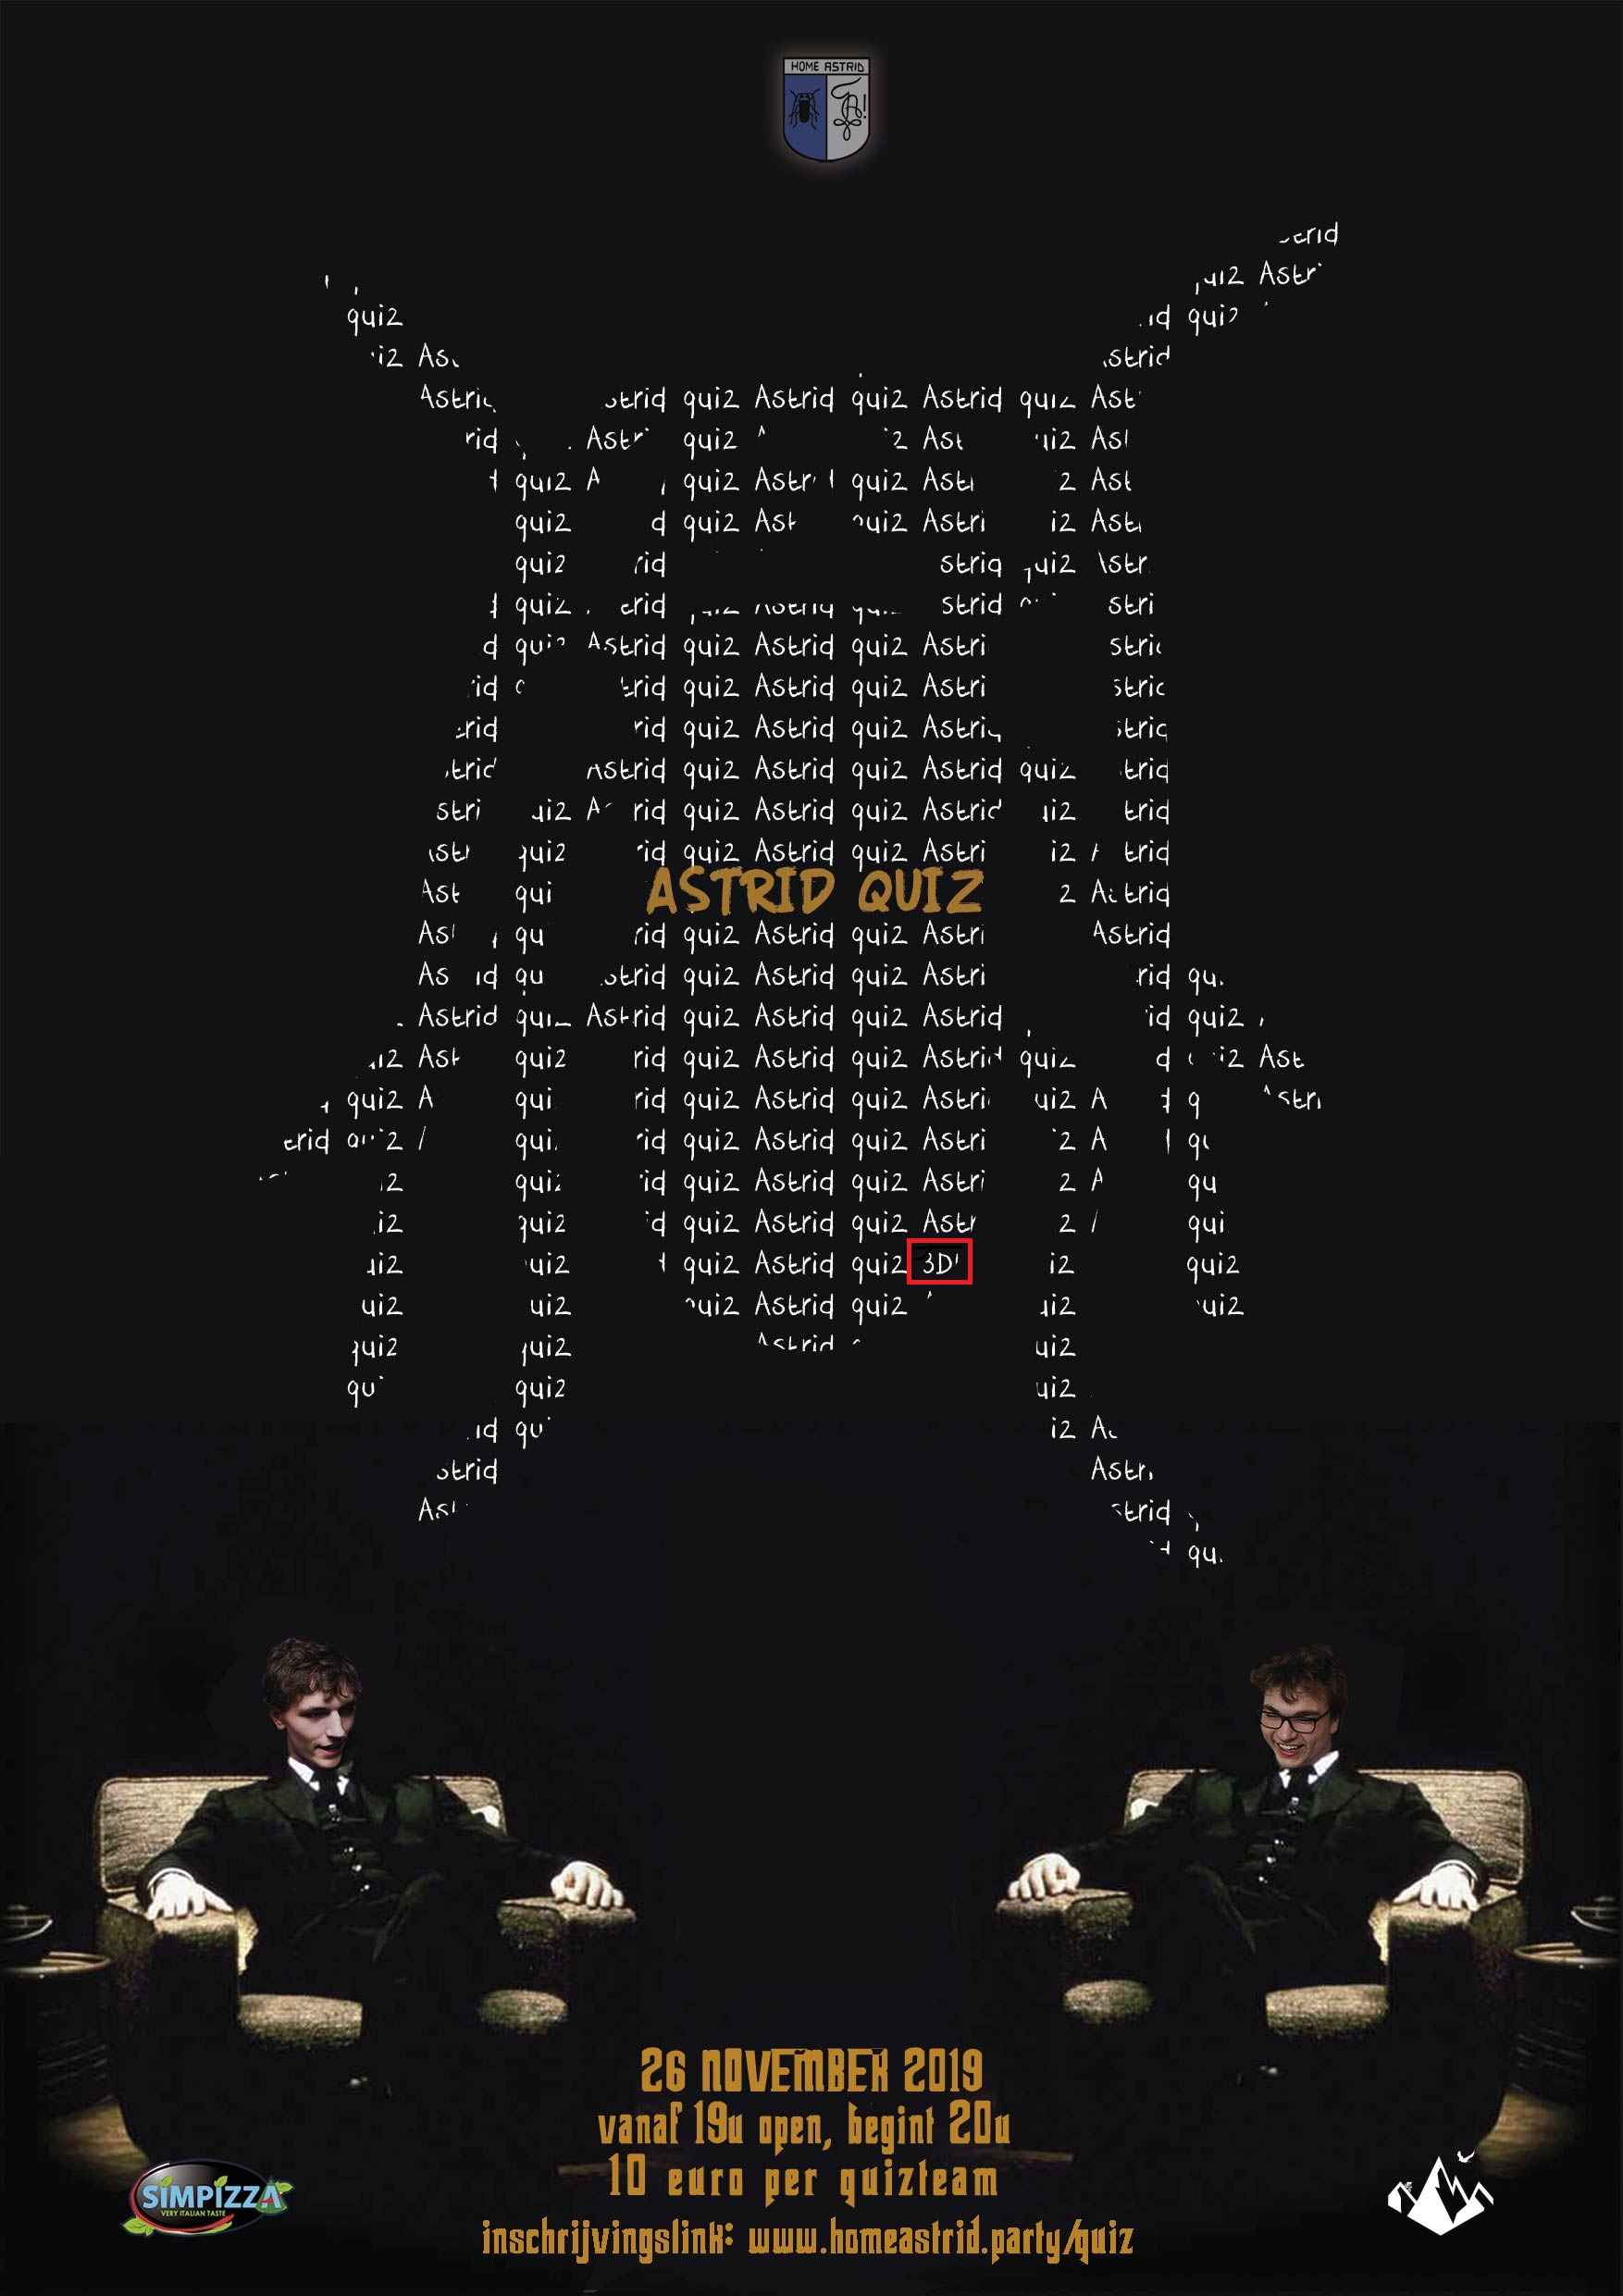
\includegraphics[scale=0.35]{quiz}
\end{center}
\section{oplossing puzzel}
\begin{center}
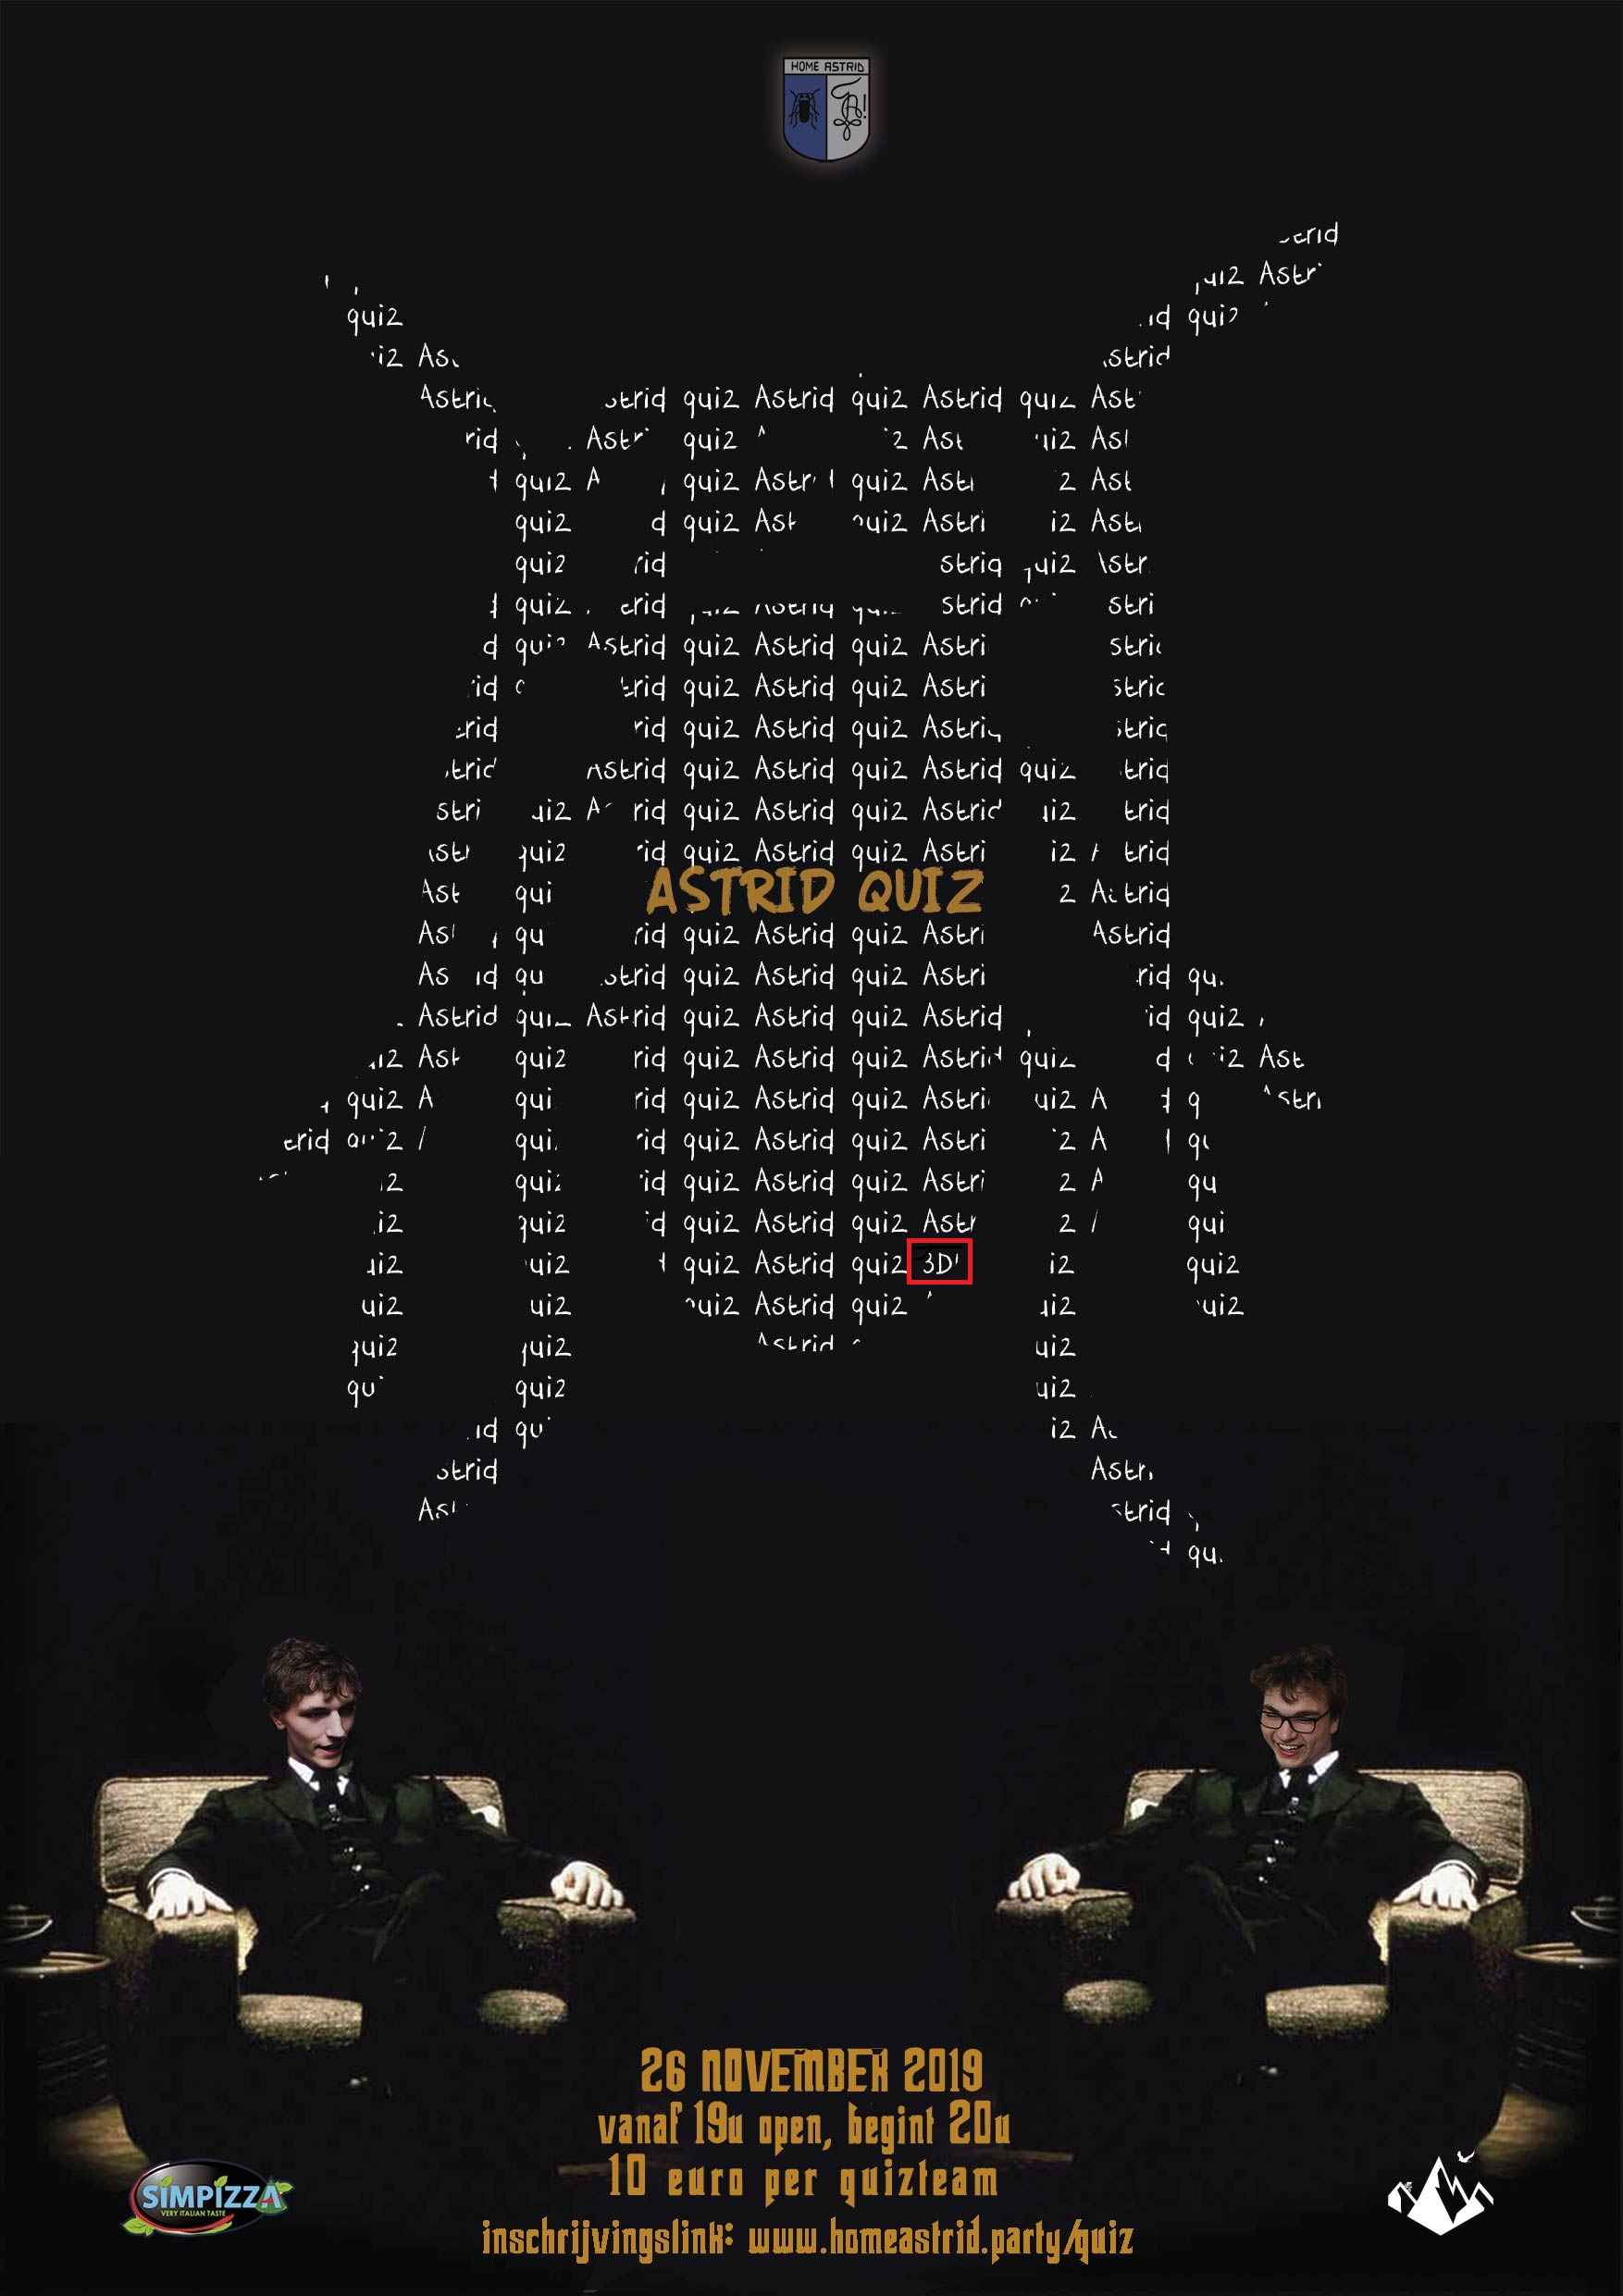
\includegraphics[scale=0.35]{quiz}
\end{center}
\end{appendices}



\end{document}